% ******************************************************** %
%              TEMPLATE DE INFORME ORGA2 v0.1              %
% ******************************************************** %
% ******************************************************** %
%                                                          %
% ALGUNOS PAQUETES REQUERIDOS (EN UBUNTU):                 %
% ========================================
%                                                          %
% texlive-latex-base                                       %
% texlive-latex-recommended                                %
% texlive-fonts-recommended                                %
% texlive-latex-extra?                                     %
% texlive-lang-spanish (en ubuntu 13.10)                   %
% ******************************************************** %


\documentclass[a4paper]{article}
\usepackage[spanish]{babel}
\usepackage[utf8]{inputenc}
\usepackage{charter}   % tipografia
\usepackage{graphicx}
\usepackage{subfig}
%\usepackage{makeidx}
\usepackage{paralist} %itemize inline

%\usepackage{float}
%\usepackage{amsmath, amsthm, amssymb}
%\usepackage{amsfonts}
%\usepackage{sectsty}
%\usepackage{charter}
%\usepackage{wrapfig}
%\usepackage{listings}
%\lstset{language=C}

% \setcounter{secnumdepth}{2}
\usepackage{underscore}
\usepackage{caratula}
\usepackage{url}


% ********************************************************* %
% ~~~~~~~~              Code snippets             ~~~~~~~~~ %
% ********************************************************* %

\usepackage{color} % para snipets de codigo coloreados
\usepackage{fancybox}  % para el sbox de los snipets de codigo

\definecolor{litegrey}{gray}{0.94}

\newenvironment{codesnippet}{%
	\begin{Sbox}\begin{minipage}{\textwidth}\sffamily\small}%
	{\end{minipage}\end{Sbox}%
		\begin{center}%
		\vspace{-0.4cm}\colorbox{litegrey}{\TheSbox}\end{center}\vspace{0.3cm}}



% ********************************************************* %
% ~~~~~~~~         Formato de las páginas         ~~~~~~~~~ %
% ********************************************************* %

\usepackage{fancyhdr}
\pagestyle{fancy}

%\renewcommand{\chaptermark}[1]{\markboth{#1}{}}
\renewcommand{\sectionmark}[1]{\markright{\thesection\ - #1}}

\fancyhf{}

\fancyhead[LO]{Sección \rightmark} % \thesection\ 
\fancyfoot[LO]{\small{Nombre Apellido, Nombre Apellido, Nombre Apellido}}
\fancyfoot[RO]{\thepage}
\renewcommand{\headrulewidth}{0.5pt}
\renewcommand{\footrulewidth}{0.5pt}
\setlength{\hoffset}{-0.8in}
\setlength{\textwidth}{16cm}
%\setlength{\hoffset}{-1.1cm}
%\setlength{\textwidth}{16cm}
\setlength{\headsep}{0.5cm}
\setlength{\textheight}{25cm}
\setlength{\voffset}{-0.7in}
\setlength{\headwidth}{\textwidth}
\setlength{\headheight}{13.1pt}

\renewcommand{\baselinestretch}{1.1}  % line spacing

% ******************************************************** %


\begin{document}


\thispagestyle{empty}
\materia{Organizacion del Computador II}
\submateria{Segundo Cuatrimestre de 2014}
\titulo{Trabajo Practico II}
\subtitulo{A PC regalado, no se le mira procesador}
\integrante{Rodrigo Kapobel}{695/12}{rok_35@live.com.ar}
\integrante{Nicolas Hernandez}{122/13}{nicoh22@hotmail.com}
\integrante{Luciano Saenz}{904/13}{saenzluciano@gmail.com}

\maketitle
\newpage

\thispagestyle{empty}
\vfill
\begin{abstract}
El presente informe tiene como objetivo implementar e investigar la eficiencia de diferentes tipos de filtros de imagenes mediante el uso del lenguaje de instrucciones assembler SIMD de intel. 
La problematica principal se basa en tratar de mostrar porque SIMD supone una mejora frente a implementaciones en otros lenguajes de mas alto nivel como puede ser C. 
\end{abstract}

\thispagestyle{empty}
\vspace{3cm}
\tableofcontents
\newpage


%\normalsize
\newpage

\section{Introducción}
Este trabajo practico consiste en dos parte: 
Una primera parte donde utilizando el modelo de procesamiento SIMD aplicamos distintos filtros sobre imagenes. Estos filtros son implementado en dos tipos de lenguaje: lenguajc y assembler.
La tecnica de SIMD nos permite aplicar una misma funcion sobre varios datos en forma vectorizada

\section{Desarrollo}
\subsection{Imágenes}

Las siguientes implementaciones operan con imágenes del tipo bmp y canales $alfa$, $red$, $green$ y $blue$ ($argb$) de 8 bits cada uno (de ahí la variante bmp 32 bits).\\

En memoria los datos de cada pixel estarán ordenados a la inversa, es decir, $bgra$, por lo cual al trabajarlos en registros de procesador, los mismos serán invertidos debido a que es el formato standard utilizado por la arquitectura intel para almacenar datos en memoria.
El puntero de fuente obtenido en todas las implementaciones representa a la imágen a la cual se le quiere aplicar el filtro. La misma tiene una particularidad para la lectura y es que la primera fila leida es la última de la imágen.\\

Llamaremos $O$ a la imágen de salida generada por cada filtro. Por ejemplo, el filtro identidad
estaría caracterizado por la fórmula\\

\begin{center}
$\forall$ $k$ $\in$ ($r, g, b, a$) $O^{k}_{i,j}$ = $I^{k}_{i,j}$
\end{center}

\subsection{Implementaciones}
Introduciremos cada filtro mencionandolos en el siguiente orden:
 
\begin{enumerate}
\item Cropflip
\item Sepia
\item Low dynamic range 
\end{enumerate}

Para cada uno expondremos su idea principal, es decir, que efecto tiene sobre la imágen a la que se aplica, mostrando un caso de ejemplo. Luego expondremos las implementaciones, focalizando y detallando principalmente la implementación en lenguaje assembler SIMD.

\subsection{Cropflip}
Este filtro es una unión de dos filtros: crop y vertical-flip. Al aplicarlo sobre una imágen, recorta una parte de la misma y la voltea verticalmente. Para ello recibe cuatro argumentos delimitando un rectangulo de la imágen.

\begin{itemize}
\item{$tamx$: Posee la cantidad de columnas, en pixeles, a recortar. Este número es multiplo de 4.}
\item{$tamy$: Contiene la cantidad de filas, en pixeles, a recortar.}
\item{$offseex$: Columna, en pixeles, a partir de la cual se debe comenzar a recortar. Este número también es multiplo de 4.}
\item{$offsety$: Fila, en pixeles, a partir de la cual se debe comenzar a recortar.}
\end{itemize}

El recuadro obtenido se devuelve espejadolo verticalmente. Para ello rearma las filas en orden inverso.\\

\newpage

\begin{figure}
  \centering
  \subfloat[Original]{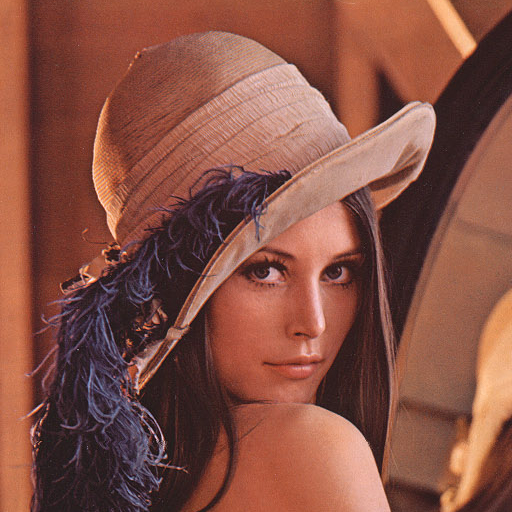
\includegraphics[width=0.4\textwidth]{imagenes/lena32.jpg}\label{fig:f1}}
  \hfill
  \subfloat[Cropflip]{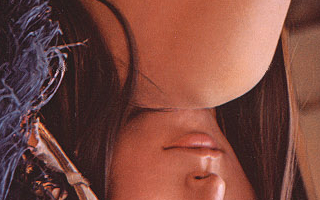
\includegraphics[width=0.4\textwidth]{imagenes/lena32cropflip.jpg}\label{fig:f2}}
  \caption{Corte: 320x200 $offset x: 100$ y $offset y: 0$}
\end{figure}

Si bien es el código más sencillo de implementar, incluso de manera eficiente, requiere algún tipo de explicación.

\subsubsection{Assembler SIMD}

En la implementación de SIMD se aprovecha el uso de paralelismo y la capacidad de almacenar hasta cuatro pixeles en un registro $xmm$.\\ 
Tomando entonces de a 4 pixeles, desde el inicio del rectangulo determinado por los parametros, se rearma la imágen, logrando finalmente, al recorrer todas las filas indicadas, el espejado vertical esperado.

\begin{codesnippet}
\begin{verbatim}
.ciclo:
        movdqu xmm1, [rdi]      ; p0|p1|p2|p3
        movdqu [rsi], xmm1
    
        lea rsi, [rsi + 16]
        lea rdi, [rdi + 16]
        loop .ciclo
\end{verbatim}
\end{codesnippet}

Como puede observarse, mediante un ciclo podemos con la ayuda de un registro xmm transportar desde la fuente hasta el destino, 4 pixeles simultaneamente, que corresponde en total a la fila de la imágen.

\subsubsection{C}

En principio, C compilado sin flags de optimización (es decir compilado con $O0$, modo default) el código final se resuelve puramente con instrucciones de assembler. Por lo tanto cada pixel se opera unitariamente. 

\begin{codesnippet}
\begin{verbatim}
    for (int i = 0; i < tamy; i++) 
    {
        for (int j = 0; j < tamx; j++) 
        {

            bgra_t *p_d = (bgra_t*) &dst_matrix[(tamy-1)-i][j*4];
            bgra_t *p_s = (bgra_t*) &src_matrix[i+offsety][(j+offsetx)*4];

            p_d->b = p_s->b;
            p_d->g = p_s->g;
            p_d->r = p_s->r;
            p_d->a = p_s->a;

        }
    }
\end{verbatim}
\end{codesnippet}

\subsection{Sepia}
Esta operación consiste en cambiar la información de color de cada pixel de la siguiente manera:

\begin{center}
$$O_{i,j}^{R} = 0, 5 . suma_{i,j}$$
$$O_{i,j}^{G} = 0, 3 . suma_{i,j}$$
$$O_{i,j}^{B} = 0, 2 . suma_{i,j}$$
\end{center}

donde 

\begin{center}
$suma_{i,j} = I_{i,j}^{R} + I_{i,j}^{G} + I_{i,j}^{B}$
\end{center}

El efecto logrado es que realza más el canal verde. 

\newpage

\begin{figure}
  \centering
  \subfloat[Original]{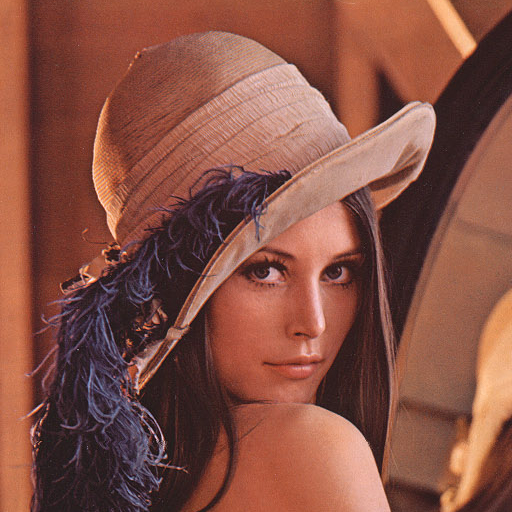
\includegraphics[width=0.4\textwidth]{imagenes/lena32.jpg}\label{fig:f3}}
  \hfill
  \subfloat[Sepia]{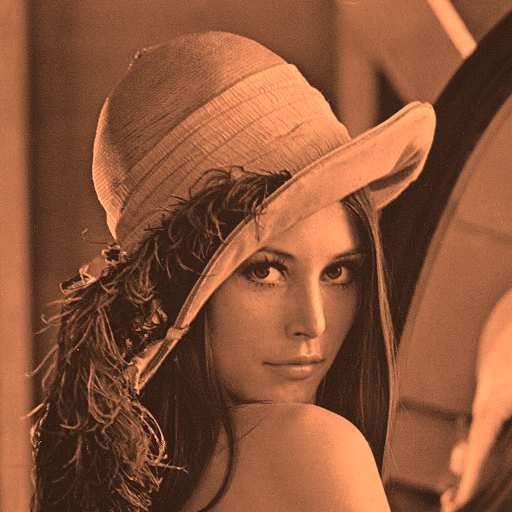
\includegraphics[width=0.4\textwidth]{imagenes/lena32sepia.jpg}\label{fig:f4}}
\end{figure}

Si bien es una operación sencilla, los tiempos de cómputo se ven comprometidos para imágenes muy grandes debido a la cantidad de operaciones en punto flotante: En una imágen de 512x512 pixeles tenemos 512x512x3 = 786432 operaciones de punto flotante. Lo cual puede suponer un desafio si no se dispone de tecnologias como SIMD.

\subsubsection{Assembler SIMD}

Al igual que en el primer filtro, se aprovecha el paralelismo de SIMD para el cálculo en punto flotante.\\

Para operar la imágen se procesa de a 4 pixeles. Luego cada pixel se lleva a un registro $xmm$ extendiendo sus canales a 32 bits. Como no se asume que el alfa sea cero se utiliza una máscara para borrarlo previemente. Luego se realiza la suma de los canales para cada pixel y por último se convierte cada una a punto flotante 32 bits y se realizan los 3 productos para cada suma que corresponden a los nuevos canales $r$, $g$ y $b$ mediante el uso de operaciones de punto flotante.\\

Al final se restaura el canal alfa junto con el nuevo pixel calculado y se devuelve a la imágen destino. 

\begin{codesnippet}
\begin{verbatim}
        movdqu xmm1, [rdi]; XMM1 = | p3 | p2 | p1 | p0 |
        movdqu xmm2, xmm1 ; XMM1 = XMM2
        movdqu xmm5, xmm1; respaldo XMM5 = XMM1

        limpiar alfa
        pand xmm1, xmm7; XMM1 = | 0 | r3 | g3 | b3 |...
        pand xmm2, xmm7; idem
        
        
        punpcklbw xmm1, xmm6; XMM1 = | p1 | p0 | con alfa limpio
        punpckhbw xmm2, xmm6; XMM2 = | p3 | p2 | con alfa limpio
        
        movdqu xmm3, xmm1
        movdqu xmm4, xmm2
        punpcklbw xmm1, xmm6; XMM1 = | 0 | r0 | g0 | b0 |
        punpckhbw xmm3, xmm6; XMM3 = | 0 | r1 | g1 | b1 |
        punpcklbw xmm2, xmm6; XMM2 = | 0 | r2 | g2 | b2 |
        punpckhbw xmm4, xmm6; XMM4 = | 0 | r3 | g3 | b3 |
        
        phaddd xmm1, xmm1; XMM1 = | r0 | g0 + b0 | r0 | g0 + b0 |
        phaddd xmm1, xmm1; XMM1 = | suma0 | suma0 | suma0 | suma0 | 
        phaddd xmm2, xmm2; idem con pixeles 1, 2 y 3
        phaddd xmm2, xmm2
        phaddd xmm3, xmm3 
        phaddd xmm3, xmm3
        phaddd xmm4, xmm4
        phaddd xmm4, xmm4

        ; un unpack mas, multiplico de a un pixel

        cvtdq2ps xmm1, xmm1;  suma0 asFloat
        cvtdq2ps xmm2, xmm2;  suma2 asFloat
        cvtdq2ps xmm3, xmm3;  suma1 asFloat
        cvtdq2ps xmm4, xmm4;  suma3 asFloat

        movups xmm0, [factores]

        mulps xmm1, xmm0; XMM1 = |*|suma0*0.2|suma0*0.3|suma0*0.5|  
        mulps xmm2, xmm0; XMM2 = |*|suma2*0.2|suma2*0.3|suma2*0.5|  
        mulps xmm3, xmm0; XMM3 = |*|suma1*0.2|suma1*0.3|suma1*0.5|   
        mulps xmm4, xmm0; XMM4 = |*|suma3*0.2|suma3*0.3|suma3*0.5|   

        cvttps2dq xmm1, xmm1; |0|suma0*0.2 asInt|suma0*0.3 asInt|suma0*0.5 asInt|
        cvttps2dq xmm2, xmm2
        cvttps2dq xmm3, xmm3
        cvttps2dq xmm4, xmm4

        packusdw xmm1, xmm3; 
        packusdw xmm2, xmm4;
        packuswb xmm1, xmm2; XMM1 = | p3' | p2' | p1'| p0'|

        ; restaurar canal alfa
        pand xmm5, xmm8
        paddb xmm1, xmm5
\end{verbatim}
\end{codesnippet}

\subsubsection{C}

Como sucede en $cropflip$, sin flags de optimización el codigo compilado con $O0$ no dispone de las ventajas de SIMD.

\begin{codesnippet}
\begin{verbatim}

    for (int i = 0; i < filas; i++)
    {
        for (int j = 0; j < cols; j++)
        {
            bgra_t *p_d = (bgra_t*) &dst_matrix[i][j * 4];
            bgra_t *p_s = (bgra_t*) &src_matrix[i][j * 4];
            aux = (int) p_s->r + (int) p_s->g + (int) p_s->b;
            p_d->r = (aux * 0.5 > 255)? 255 : aux * 0.5;
            p_d->g = (aux * 0.3 > 255)? 255 : aux * 0.3;
            p_d->b = (aux * 0.2 > 255)? 255 : aux * 0.2;
            p_d->a = p_s->a;
        }
    }

\end{verbatim}
\end{codesnippet}


\subsection{LDR: Low Dynamic Range}

El filtro $ldr$ es el que más operaciones lleva a cabo de los tres.
Toma una imágen y aplica un efecto que modifica la imagen según su iluminación. El filtro toma el valor de un pixel y le añade un porcentaje $\alpha$ del de sus vecinos.\\

De esta manera, dado un porcentaje positivo, los pixeles rodeados por pixeles claros se vuelven
aún más claros, mientras que los rodeados por pixeles oscuros se mantienen igual. La intensidad
del efecto dependerá del porcentaje sumado.
Para cada componente independiente del pixel ($r$, $g$ y $b$) la fórmula matemática será:

\begin{center}
$$O_{i,j}^{K} = min(max(ldr_{i,j}^{K},0),255)$$
\end{center}

donde

\begin{center}
$$ldr_{i,j}^{K} = I_{i,j}^{K} + \alpha \frac{sumargb_{i,j}}{max} . I_{i,j}^{K}$$
$$sumargb_{i,j} = suma_{i,j}^{r} + suma_{i,j}^{g} + suma_{i,j}^{b}$$
$$max = 5*5*255*3*255$$
\end{center}

255 y 0 corresponden a valores de saturación y finalmente $suma_{i,j}^{K}$ corresponde a:

\begin{center}
$I_{i+2,j-2}^{K}$ + $I_{i+2,j-1}^{K}$ + $I_{i+2,j}^{K}$ + $I_{i+2,j+1}^{K}$ + $I_{i+2,j+2}^{K}$ +\\
$I_{i+1,j-2}^{K}$ + $I_{i+1,j-1}^{K}$ + $I_{i+1,j}^{K}$ + $I_{i+1,j+1}^{K}$ + $I_{i+1,j+2}^{K}$ +\\
$I_{i,j-2}^{K}$ + $I_{i,j-1}^{K}$ + $I_{i,j}^{K}$ + $I_{i,j+1}^{K}$ + $I_{i,j+2}^{K}$ +\\
$I_{i-1,j-2}^{K}$ + $I_{i,j-1}^{K}$ + $I_{i-1,j}^{K}$ + $I_{i-1,j+1}^{K}$ + $I_{i-1,j+2}^{K}$ +\\ 
$I_{i-2,j-2}^{K}$ + $I_{i-2,j-1}^{K}$ + $I_{i-2,j}^{K}$ + $I_{i-2,j+1}^{K}$ + $I_{i-2,j+2}^{K}$ +\\
\end{center}

\newpage

\begin{figure}
  \centering
  \subfloat[Original]{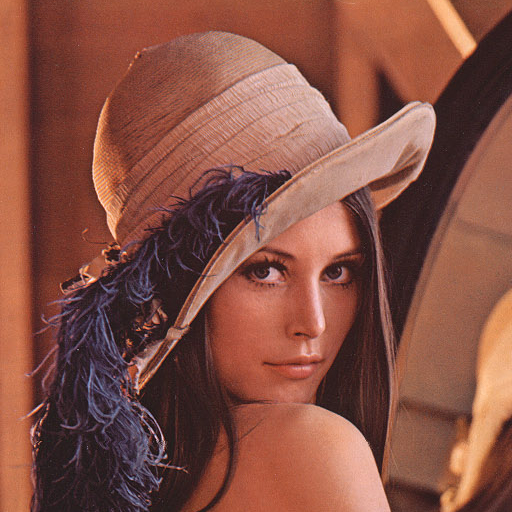
\includegraphics[width=0.4\textwidth]{imagenes/lena32.jpg}\label{fig:f5}}
  \hfill
  \subfloat[LDR]{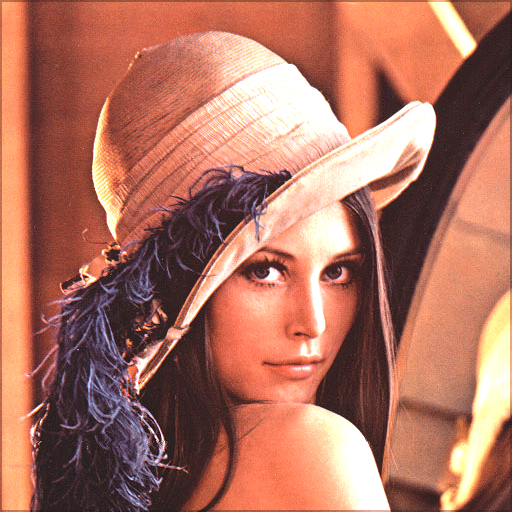
\includegraphics[width=0.4\textwidth]{imagenes/lena32ldr.jpg}\label{fig:f6}}
  \caption{$\alpha$: 255}
\end{figure}


Para reducir errores de redondeo, la division debe será la última operación en realizarse.
El resultado final será saturado de ahi $max$ y $min$ en la primer fórmula.

Además, dado que en los bordes no es posible calcular $ldr$ por la ausencia de vecinos, se devolverá
el valor original. Es decir:

\begin{center}
$O_{i,j}^{K} = I_{i,j}^{K}$ si $i<2 \vee j<2 \vee i+2 \leq tamy \vee j +2 \leq tmax$
\end{center}

(con i indexado a partir de 0)

\subsubsection{Assembler SIMD}

En la implementación de $ldr$ tenemos varios inconvenientes a solventar, pero el principal es el cálculo de la suma. Para lograr aprovechar el paralelismo que ofrece SIMD se realizan varias operaciones.
Para cada fila del cuadrado que supone la sumatoria, se obtienen 4 pixeles en un registro $xmm$ y luego se separan en dos registros diferentes, de manera tal que tengamos el los pixeles $p0$ y $p1$ en uno y $p2$ y $p3$ en otro con cada canal transformado a 16 bits. Para realizarlo se realiza un shuffle para cada caso.\\

Una vez obtenidos los dos registros anteriores, se suman horizontalmente los registros respectivos una vez y se transforma el resultado a 32 bits. Luego se aplican sumas verticales valiendose de un registro de respaldo y varios shifts para eliminar las sumas que no signifiquen en la fórmula.\\

Debido a que la suma que buscamos es de cinco pixeles, se obtiene el 5to pixel en otro registro y se lo opera de manera similar a los anteriores para luego sumarlo a los mismos acumulando la suma de cada fila en el registro particular $xmm0$

\begin{codesnippet}
\begin{verbatim}
.cincoHorizontal:

    ; 16  12   8   4   0
    ; Li4|Li3|Li2|Li1|Li0
    ;VERSION STANDARD: Con 2 accesos - acceso extra paa el pixel 5
    movdqu xmm13, [rdi + r12*pixelSize] ; Li3|Li2|Li1|Li0

    movdqu xmm9, xmm13
    pshufb xmm9, xmm6 ; 0|0|0|r1|0|g1|0|b1|0|0|0|r0|0|g0|0|b0
    phaddw xmm9, xmm11 ; 0|0|0|0|0+r1|g1+b1|0+r0|g0+b0 
    pshufb xmm13, xmm7 ; 0|0|0|r3|0|g3|0|b3|0|0|0|r2|0|g2|0|b2
    phaddw xmm13, xmm11 ; 0|0|0|0|r3|g3+b3|r2|g2+b2 
    punpcklwd xmm9, xmm11 ; r1|g1+b1|r0|g0+b0
    punpcklwd xmm13, xmm11 ; r3|g3+b3|r2|g2+b2
    paddd xmm13, xmm9 ; r3+r1|g3+b3+g1+b1|r2+r0|g2+b2+g0+b0 
    movdqu xmm9, xmm13
    psrldq xmm9, 8 ; 0|0|r3+r1|g3+b3+g1+b1
    paddd xmm13, xmm9 ; r3+r1|g3+b3+g1+b1|r2+r0+r3+r1|g2+b2+g0+b0+g3+b3+g1+b1 
    pslldq xmm13, 8 ; r2+r0+r3+r1|g2+b2+g0+b0+g3+b3+g1+b1|0|0
    psrldq xmm13, 8 ; 0|0|r2+r0+r3+r1|g2+b2+g0+b0+g3+b3+g1+b1
    movd xmm9, [rdi + r12*pixelSize + 16] ; 0|0|0|0|0|0|0|0|0|0|0|0|a4|r4|g4|b4

    pslldq xmm9, 12 ; a4|r4|g4|b4|0|0|0|0|0|0|0|0|0|0|0|0
    pand xmm9, xmm8 ; 0|r4|g4|b4|0|0|0|0|0|0|0|0|0|0|0|0
    pshufb xmm9, xmm7 ; 0|0|0|r4|0|g4|0|b4|0|0|0|0|0|0|0|0
    phaddw xmm9, xmm11 ; 0|0|0|0|r4|g4+b4|0|0 -- maximo por w = 510 in []
    punpcklwd xmm9, xmm11 ; 0|r4|0|g4+b4|0|0|0|0
    psrldq xmm9, 8 ; 0|0|r4|g4+b4
    paddd xmm13, xmm9 ; 0|0|r2+r0+r3+r1+r4|g2+b2+g0+b0+g3+b3+g1+b1+g4+b4 
    movdqu xmm9, xmm13
    psrldq xmm9, 4 ; 0|0|0|r2+r0+r3+r1+r4
    paddd xmm13, xmm9 ; 0|0|r2+r0+r3+r1+r4|g2+b2+g0+b0+g3+b3+g1+b1+g4+b4+r2+r0+r3+r1+r4 
    pslldq xmm13, 12 ; g2+b2+g0+b0+g3+b3+g1+b1+g4+b4+r2+r0+r3+r1+r4|0|0|0
    psrldq xmm13, 12 ; 0|0|0|g2+b2+g0+b0+g3+b3+g1+b1+g4+b4+r2+r0+r3+r1+r4
    paddd xmm0, xmm13 ; suma de la i fila para el pixel ij.

    add r12, r15
    inc r10
    cmp r10, 5
    jl .cincoHorizontal
    
\end{verbatim}
\end{codesnippet}

Una vez obtenida la suma, que al final tendrá un tamaño de 32 bits, se procede a realizar la fórmula de $ldr$. 
El primer paso es armar la un registro con el valor de $alfa$ en sus primeras tres posiciones menos significativas que es donde se encontraran los valores de los canales. Asi mismo, se crea un registro con el divisor $max$ en las cuatro posiciones debido a que con el realizaremos la division.\\

Se crea un registro con la suma replicada en las tres posiciones menos significativas y se procede a calcular la fórmula, para lo cual tenemos la siguiente consideración:\\
 
Debido a que, $canal x sumargb x alfa$ cabe perfectamente dentro de un entero de 32 bits (el máximo es 75x255x255x255 o 75x255x255x-255 = +-1,243,603,125 $\in$ $[$-2,147,483,648 a 2,147,483,647$]$, no se convierte a punto flotante si no hasta la division, por lo tanto será la única operacion de punto flotante del algoritmo, aunque vale mencionar que si por cada pixel, exceptuando las primeras y últimas dos filas y columnas se aplica esta fórmula en total habrá 3x(filas-2)x(columnas-2) operaciones de punto flotante. Para una imágen de 512$x$512 supone 780300 divisiones de punto flotante, que se asemeja bastante a la cantidad de operaciones de punto flotante de $sepia$.


\begin{codesnippet}
\begin{verbatim}
    
    pxor xmm13, xmm13
    movd xmm13, ebx
    movdqu xmm12, xmm13 ; 0|0|0|alpha
    pslldq xmm12, 4 ; 0|0|alpha|0
    por xmm12, xmm13 ; 0|0|alpha|alpha
    pslldq xmm12, 4 ; 0|alpha|alpha|0
    por xmm12, xmm13 ; 0|alpha|alpha|alpha

    pxor xmm14, xmm14
    movd xmm14, r13d
    movdqu xmm13, xmm14 ; 0|0|0|max
    pslldq xmm13, 4 ; 0|0|max|0
    por xmm13, xmm14 ; 0|0|max|max
    pslldq xmm13, 4 ; 0|max|max|0
    por xmm13, xmm14 ; 0|max|max|max
    pslldq xmm13, 4 ; max|max|max|0
    por xmm13, xmm14 ; max|max|max|max

    movdqu xmm5, xmm0 0|0|0|0
    pslldq xmm5, 4 0|0|sumargb|0
    por xmm5, xmm0 0|0|sumargb|sumargb
    pslldq xmm5, 4 0|sumargb|sumargb|0
    por xmm5, xmm0 0|sumargb|sumargb|sumargb
    pxor xmm14, xmm14
    movd xmm14, [rdi + r8*pixelSize] ; 0|0|0|0|0|0|0|0|0|0|0|0|a|r|g|b <- get pixel ij
    movdqu xmm0, xmm14 ; 0|0|0|0|0|0|0|0|0|0|0|0|a|r|g|b
    pand xmm0, xmm15 ; 0|0|0|0|0|0|0|0|0|0|0|0|0|r|g|b
    punpcklbw xmm0, xmm11 ; 0|0|0|0|0|r|g|b
    punpcklwd xmm0, xmm11 ; 0|r|g|b
    ; 0|sumargb*r|sumargb*g|sumargb*b == 0|sumargb*r|sumargb*g|sumargb*b
    pmulld xmm5, xmm0 
    ; puede cambiar el signo segun alpha
    ; 0|alpha*sumargb*r|alpha*sumargb*g|alpha*sumargb*b 
    pmulld xmm5, xmm12 
     ; 0|fp(alpha*sumargb*r)|fp(alpha*sumargb*g)|fp(alpha*sumargb*b)
    cvtdq2ps xmm5, xmm5
    cvtdq2ps xmm13, xmm13 ; fp(max)|fp(max)|fp(max)|fp(max)
    divps xmm5, xmm13 ; 0|(alpha*sumargb*r)/max|(alpha*sumargb*g)/max|(alpha*sumargb*b)/max
    cvtdq2ps xmm0, xmm0 ; 0|fp(r)|fp(g)|fp(b)
    ; 0|r+(alpha*sumargb*r)/max|g+(alpha*sumargb*g)/max|b+(alpha*sumargb*b)/max
    addps xmm5, xmm0 
    cvttps2dq xmm5, xmm5 ; cast to dw signed 
    ; 0|0|0|0|0|r+(alpha*sumargb*r)/g+max|(alpha*sumargb*g)/b+max|(alpha*sumargb*b)/max
    packusdw xmm5, xmm11 
    packuswb xmm5, xmm11 
    ; tengo los canales calculados saturados a byte.
    ; 0|0|0|0|0|0|0|0|0|0|0|0|0|r+(alpha*sumargb*r)/g+max|(alpha*sumargb*g)/b+max|(alpha*sumargb*b)/max 
    pand xmm14, xmm4 ; 0|0|0|0|0|0|0|0|0|0|0|0|a|0|0|0
    ; 0|0|0|0|0|0|0|0|0|0|0|0|a|r+(alpha*sumargb*r)/max|g+(alpha*sumargb*g)/max|b+(alpha*sumargb*b)/max
    por xmm14, xmm5 
    
\end{verbatim}
\end{codesnippet}

\subsubsection{C}

Como ya hemos explicado, C compilado en modo default, carece de paralelismo en las operaciones y por lo tanto $ldr$ se resolverá obteniendo cada pixel y operando unitariamente. Al final el agoritmo es similar pero con más accesos a memoria para lectura y escritura y operaciones de punto flotante unitarias.

\begin{codesnippet}
\begin{verbatim}
                
                int i = 0;
                int indexSquare = c - ((cols*2)+2);
                int sumargb = 0;
                
                while (i < 5) {
                    sumargb += src[indexSquare*4];
                    sumargb += src[indexSquare*4+1];
                    sumargb += src[indexSquare*4+2];
                    sumargb += src[indexSquare*4+4];
                    sumargb += src[indexSquare*4+5];
                    sumargb += src[indexSquare*4+6];
                    sumargb += src[indexSquare*4+8];
                    sumargb += src[indexSquare*4+9];
                    sumargb += src[indexSquare*4+10];
                    sumargb += src[indexSquare*4+12];
                    sumargb += src[indexSquare*4+13];
                    sumargb += src[indexSquare*4+14];
                    sumargb += src[indexSquare*4+16];
                    sumargb += src[indexSquare*4+17];
                    sumargb += src[indexSquare*4+18];
                    indexSquare += cols; //siguiente fila.
                    i++;
                }

                float sumargbf = sumargb;
                float alphaf = alpha;
                float maxf = 4876875;
                float b = (float)src[c*4];
                float g = (float)src[c*4+1];
                float r = (float)src[c*4+2];
                unsigned char a = src[c*4+3];

                b = b + (alphaf*sumargbf*b)/maxf;

                b = MIN(MAX(b,0), 255);

                g = g + (alphaf*sumargbf*g)/maxf;

                g = MIN(MAX(g,0), 255);

                r = r + (alphaf*sumargbf*r)/maxf;

                r = MIN(MAX(r,0), 255);

                dst[c*4] = (unsigned char)b;
                dst[c*4+1] = (unsigned char)g;
                dst[c*4+2] = (unsigned char)r;
                dst[c*4+3] = a;
                
\end{verbatim}
\end{codesnippet}

\subsection{Análisis experimental}

En general, al aplicar filtros sobre imagenes, la performance puede verse afectada por varios motivos, como por ejemplo el scheduler del sistema, que puede generar caidas en el tiempo debido a que debe realizar operaciones de mayor prioridad antes de poder retornar al algoritmo.\\

Como bien se sabe, la mayoria de los procesadores poseen una memoria integrada que es la más rápida luego de los registros, conocida como memoria caché, y que se subdivide en dos niveles: L1 (a su vez subdividida en datos e instrucciones) y L2 para datos. 
La idea de la misma es tener $"$a mano$"$ datos que sean pedidos al sistema, trayendo consigo además los contiguos en un bloque de memoria (principio de vecinidad espacial), de manera tal que al consultar por el mismo nuevamente o algún contiguo, se obtenga mucho más rápido desde esta memoria. Pero cuando los mismos no se encuentran, el procesador tiene que buscarlos en la memoria ram, siendo este proceso la causa en la caida de performance que más suele afectar a los algoritmos.\\ 

Este y algunos motivos más serán de estudio en este informe. Para ello introduciremos cada una de las hipótesis que se plantearán en base a lo que cada implementación en particular genere y propondremos un test a realizar, explicando la metodologia para llevarlo a cabo y los resultados obtenidos con las conclusiones que correspondan.\\
 
Además, escogeremos una implementación en particular para llevar a cabo algunos tests especiales que surjan en base a resultados más o menos generales para tener una vision extra de lo que sucede en esos casos.\\

\subsubsection{Metodologias}

Evaluaremos con los distintos tests el rendimiento de cada implementación. El mejor o peor rendimiento de las implementaciones se basa en la toma de tiempos de ejecución. Como los tiempos de ejecución son relativamente pequeños, en general, se utilizará uno de los contadores de performance que posee el procesador. \\
Para las mediciones realizadas tomaremos una media $\alpha$-podada 0.5 sobre el total de las corridas de un experimento. La poda se realizará a derecha, eliminando así los outliers más grandes que puedan existir (las muestras se ordenan de menor a mayor). Luego tomaremos la varianza muestral, podando los datos con el mismo $\alpha$, para poder medir que dispersion tienen los mismos con respecto a la media. 
De esta manera podremos saber que si la dispersion de los datos es muy grande, para dos curvas aparentemente distanciadas en promedio, tal vez no haya diferencias sigificativas.

La imágen elegida para los tests será la siguiente:.

\newpage

\begin{figure}
  \begin{center}
	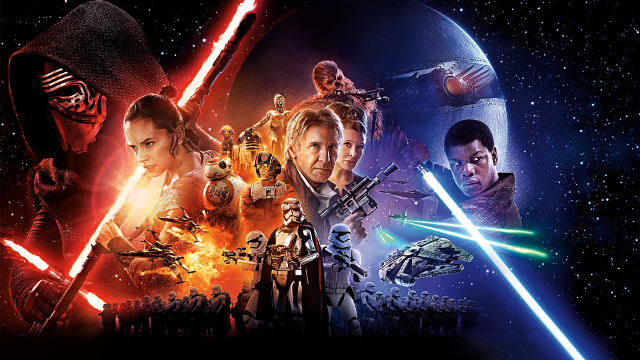
\includegraphics[scale=.5]{imagenes/starWars.jpg}
	\caption{La última de Star Wars}
	\label{starwars}
  \end{center}
\end{figure}

El procesador utilizado para realizar todos los tests sera un Intel(R) Core(TM) i5-2500K CPU @ 3.30GHz con caché L2 de 2MB.

Para que la caché no influya en cada corrida se implementó un algoritmo sencillo que lo que hará es ocupar la caché L2 antes de cada corrida. Sabiendo que la caché es de 2MB el algoritmo siguiente debería garantizar que la caché se ocupará con información que no altere los resultados de los tests. \\

\begin{codesnippet}
\begin{verbatim}
                
                char *basura = (char*)malloc(sizeof(char)*2048);
                srand(5);
                int i = 0;
                while (i < 2048) {
                    basura[i] = rand() % 27;            
                    i++;                
                }
                long int suma = 0;
                i = 0;                
                while (i < 2048) {
                    suma += basura[i];   
                    i++;         
                }
                //llamada test
                free(basura);
                
\end{verbatim}
\end{codesnippet}

\pagebreak

\subsection{Hipótesis}


\subsubsection{Comportamiento: Aumentando resoluciones}

Nos interesa saber como varia el rendimiento de los algoritmos para cada filtro en sus dos variantes ($asm$, $C$) cuando se varia el tamaño de ~\ref{starwars}. Es decir, analizaremos el comportamiento de los algoritmos frente a variaciones de tamaño\\

El resultado esperado es que para todos los filtros en ambas versiones el tiempo sea creciente a medida que el tamaño crece y si el aumento es cuadratico en el tamaño, también lo sea en el tiempo. \\
Además, que la version en implementada en $asm$ se mantenga por encima de $C$ siempre. \\ 



\subsubsection{Performance: implementaciones y filtros}

La meta principal del informe es comprobar que $asm$ es mejor que la implementación en $C$
Para esto correremos todos los filtros comparando sus versiones de $assembler$, $C$ y además incluiremos $C$ con flags de optimización, en particular $O3$ para ver que tan bien puede optimizar el compilador. \\

El resultado esperado es que $assembler$ debería ser superior, es decir insumir una menor cantidad de ciclos de reloj que las otras dos versiones. Aunque no esperariamos un mal rendimiento de $C$ con optimización. \\



\subsubsection{Performance: $cropflip$ vs. caché}

El filtro $cropflip$ parece poseer una particularidad. Utiliza accesos a memoria aleatorios que en principio deberian afectar el rendimiento en cuanto a si los datos pedidos estan cacheados o no. 
Si el corte realizado es muy ancho que alto, por principio de vecinidad espacial, el algoritmo debería tener un buen rendimiento, no así, cuando el corte es mas alto que ancho. \\

Llevaremos a cabo entonces, un test para comprobar si este hecho tiene relevancia, esperando que, verdaderamente sea un factor influyente.
Lo que haremos, como se comentó anteriormente, será limpiar la caché en cada corrida, para que así cada test no se vea afectado por el anterior. Luego esperariamos ver que cuanto más alto que ancho sea el corte peor rendimiento tendrá el algoritmo debido a que como los datos no se encuentran cacheados, tendrá más accesos a memoria ram. \\

\subsubsection{Performance: versiones de $ldr$}

Elegimos el filtro $ldr$ para analizar dos teorias relacionadas a SIMD. 

$A)$ Si igualamos la cantidad de accesos de la version de $assembler$ a la de $C$ aún asi la version de $assembler$ será más óptima.

$B)$ Si en vez de dividir en punto flotante se reemplaza esa seccion de codigo por operaciones con enteros: que version tiene mejor rendimiento? $assembler$ con ops de punto flotante o $assembler$ con ops en enteros?


\begin{codesnippet}
\begin{verbatim}
                
    ;TEST 2: OPERACIONES CON ENTEROS
    pmulld xmm5, xmm0 ; 0|sumargb*r|sumargb*g|sumargb*b == 0|sumargb*r|sumargb*g|sumargb*b
    ; puede cambiar el signo segun alpha
    pmulld xmm5, xmm12 ; 0|alpha*sumargb*r|alpha*sumargb*g|alpha*sumargb*b 
    mov r10, rdx ; salvo resto
    xor rdx, rdx
    xor rax, rax
    movd eax, xmm5 ; alpha*sumargb*b
    div r13d ; alpha*sumargb*b/max
    pxor xmm10, xmm10
    movd xmm10, eax ; 0|0|0|alpha*sumargb*b
    pslldq xmm10, 4 ; 0|0|alpha*sumargb*b|0
    xor rdx, rdx
    xor rax, rax
    psrldq xmm5, 4
    movd eax, xmm5 ; alpha*sumargb*g
    div r13d ; alpha*sumargb*g/max
    movd xmm10, eax ; 0|0|alpha*sumargb*b/max|alpha*sumargb*g/max
    pslldq xmm10, 4 ; 0|alpha*sumargb*b/max|alpha*sumargb*g/max|0
    xor rdx, rdx
    xor rax, rax
    psrldq xmm5, 4
    movd eax, xmm5 ; alpha*sumargb*r
    div r13d ; alpha*sumargb*r/max
    movd xmm10, eax ; 0|0|alpha*sumargb*b/max|alpha*sumargb*g/max|alpha*sumargb*r/max
    mov rdx, r10 ; recupero resto
                
\end{verbatim}
\end{codesnippet}



\section{Tests}

\subsection{Aumentando resoluciones}
Parámetros del test: \\
Cantidad de iteraciones por filtro 10. Aumentos 100x100.\\
$\alpha = 150$\\
Arrancamos en 1740x60 y vamos aumentando hasta 3840x2160.

\newpage

\begin{figure}
  \begin{center}
	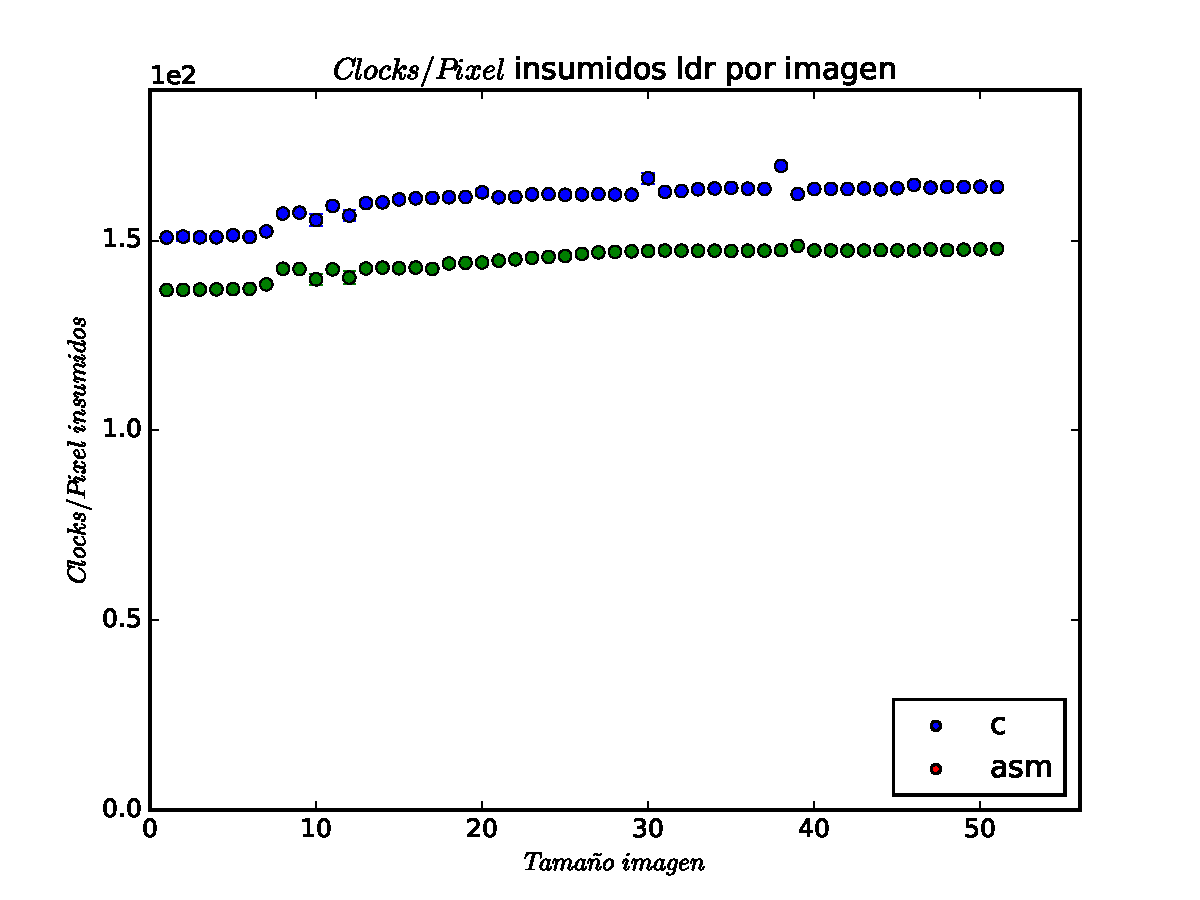
\includegraphics[scale=0.5]{ldrall.pdf}
	%\caption{La última de Star Wars}
  \end{center}
\end{figure}

\begin{figure}
  \begin{center}
	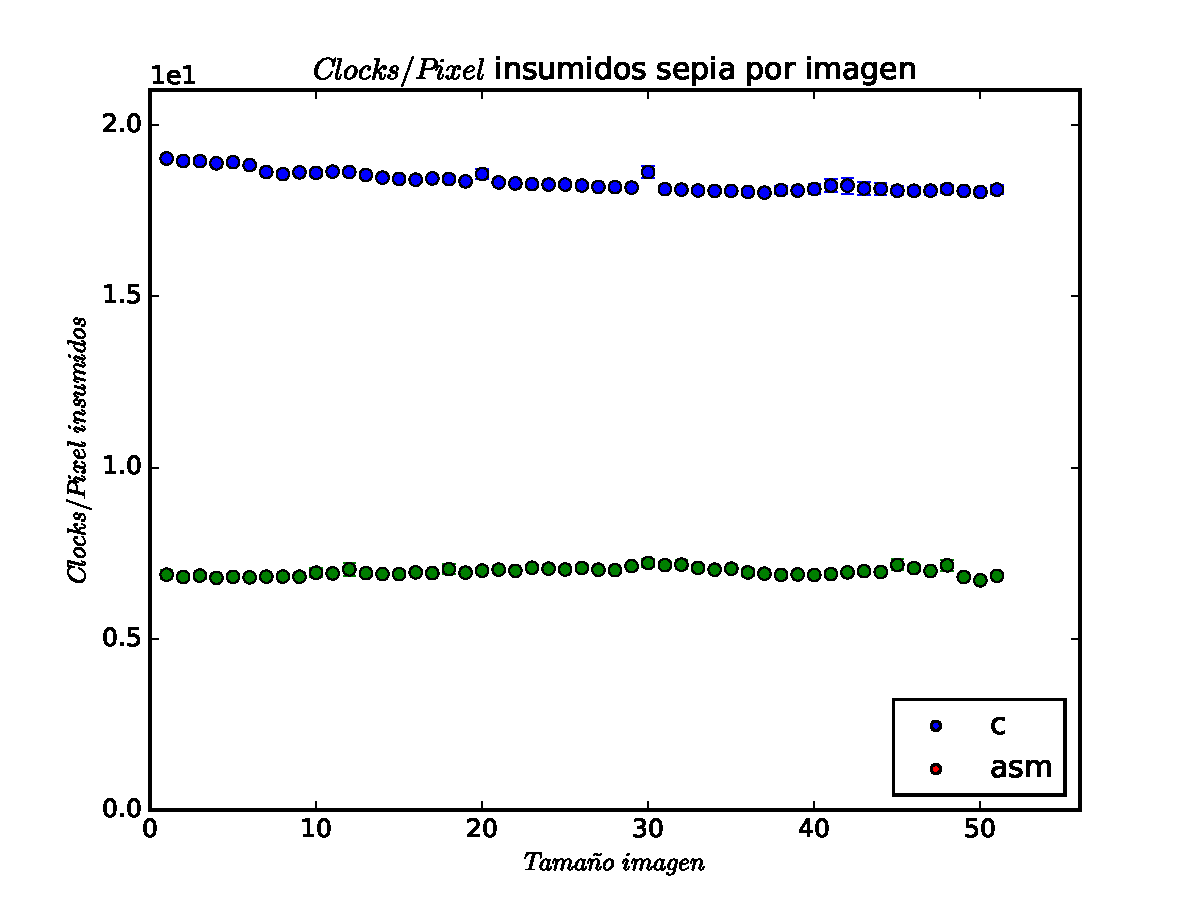
\includegraphics[scale=0.5]{sepiaall.pdf}
	%\caption{La última de Star Wars}
  \end{center}
\end{figure}


\subsubsection*{LDR Y SEPIA}  

Según nuestra hipótesis, con un aumento de forma cuadrática en el tamaño de las imágenes se obtiene una curva casi cuadratica, la curva resultante es muy parecida a una cuadratica pero con un menor crecimiento, en un principio supusimos que esto tenia que ver con que la imagen era mas ancha que alta, asi que invertimos el tamaño de la imágen original de 3840x2160 a 2160x3840 y generamos los mismos aumentos pero invertidos. El resultado obtenido es identico al original, por lo cual no tiene sentido mostrar un gráfico. Suponemos entonces que el factor de anchura o altura de la imágen en estos dos filtros no influye si aumentan los dos en iguales proporciones. \\

Luego se plantea que con dejar fijo un tamaño y aumentar el otro el resultado seria un aumento lineal de tiempos. Elegimos dejar fija la altura y aumentar el ancho desde 40x2160 a 3840x2160 y el resultado es que si, efectivamente el aumento es lineal. \\

\subsubsection*{CROPFLIP}

CORTE: 60 140 0 0 

\begin{figure}
  \begin{center}
	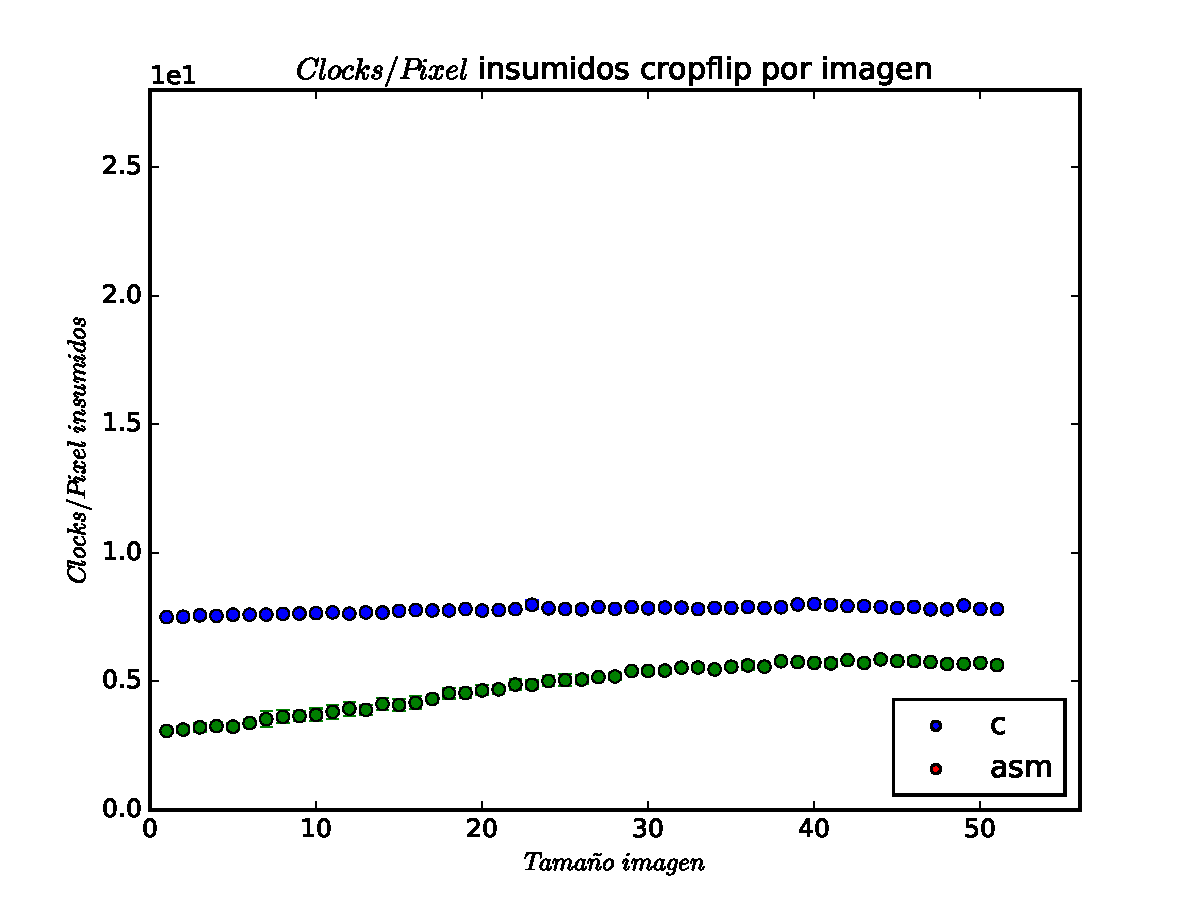
\includegraphics[scale=0.5]{cropflipall.pdf}
	%\caption{La última de Star Wars}
  \end{center}
\end{figure}


Por último observar que en cropflip se mantiene constante, es decir no cumple con lo esperado, (aunque si respeta que assembler es mejor que C). \\
\newpage

\newpage

\subsection{Performance: implementaciones y filtros}

Parámetros del test: 
Cantidad de iteraciones por filtro-version 20.

\begin{figure}[h]
  \begin{center}
	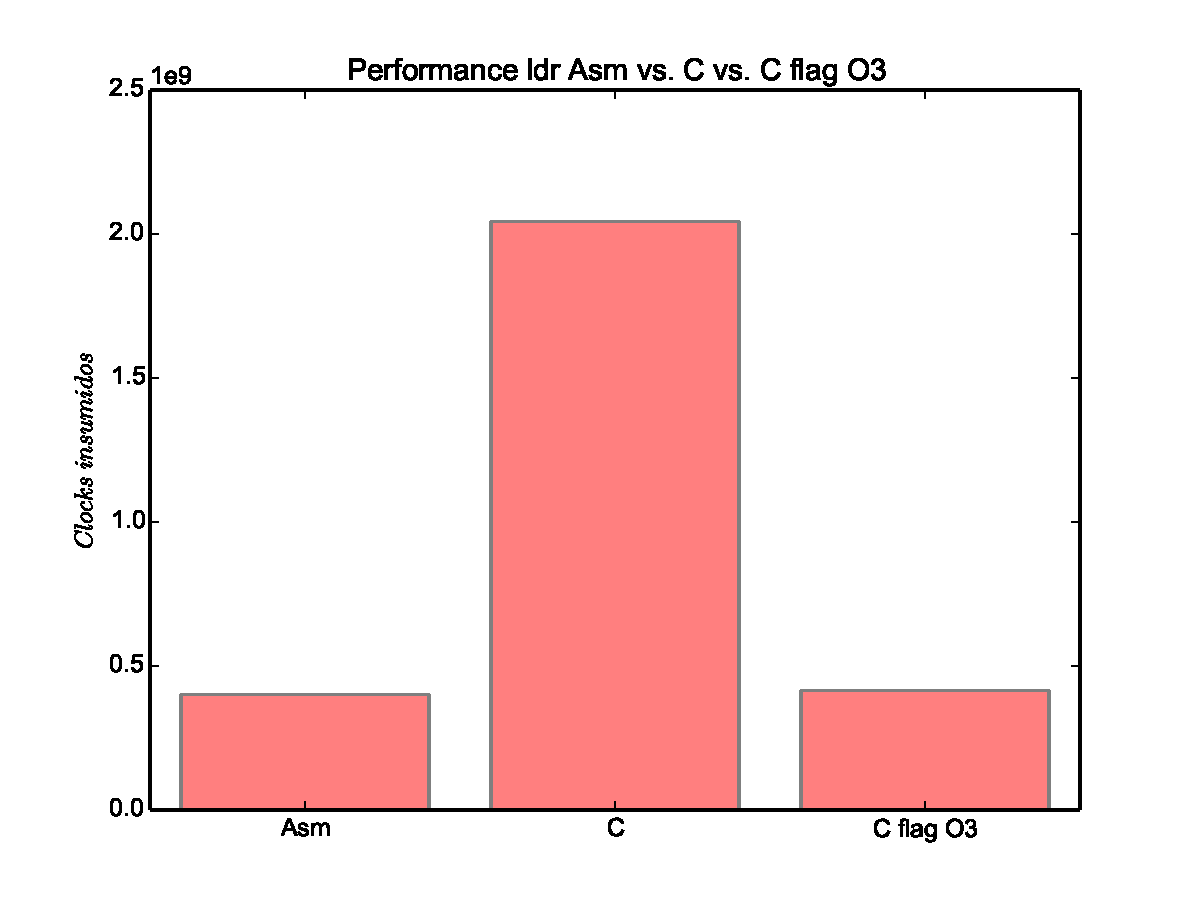
\includegraphics[scale=0.5]{ldr.pdf}
	%\caption{La última de Star Wars}
  \end{center}
\end{figure}

\begin{figure}[h]
  \begin{center}
	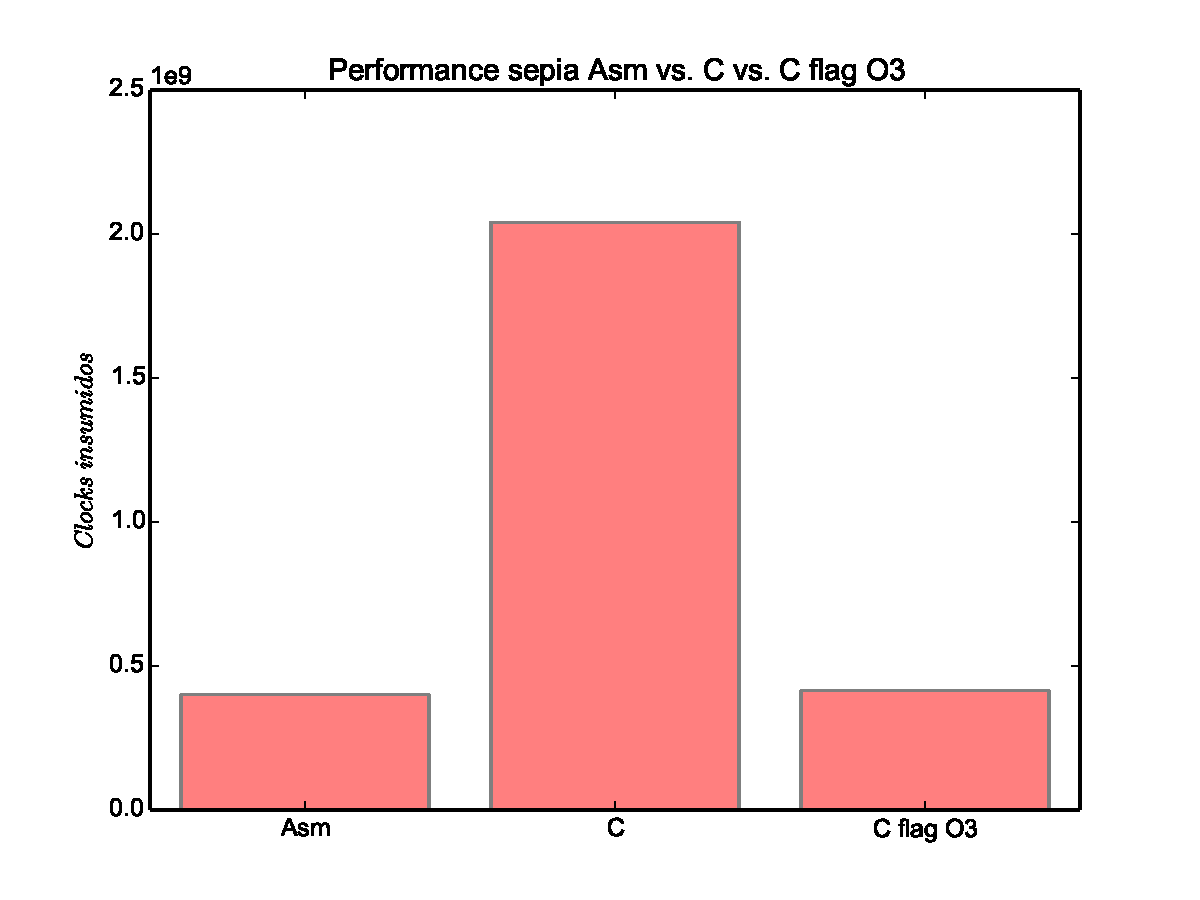
\includegraphics[scale=0.5]{sepia.pdf}
	%\caption{La última de Star Wars}
  \end{center}
\end{figure}

\newpage

\begin{figure}
  \begin{center}
	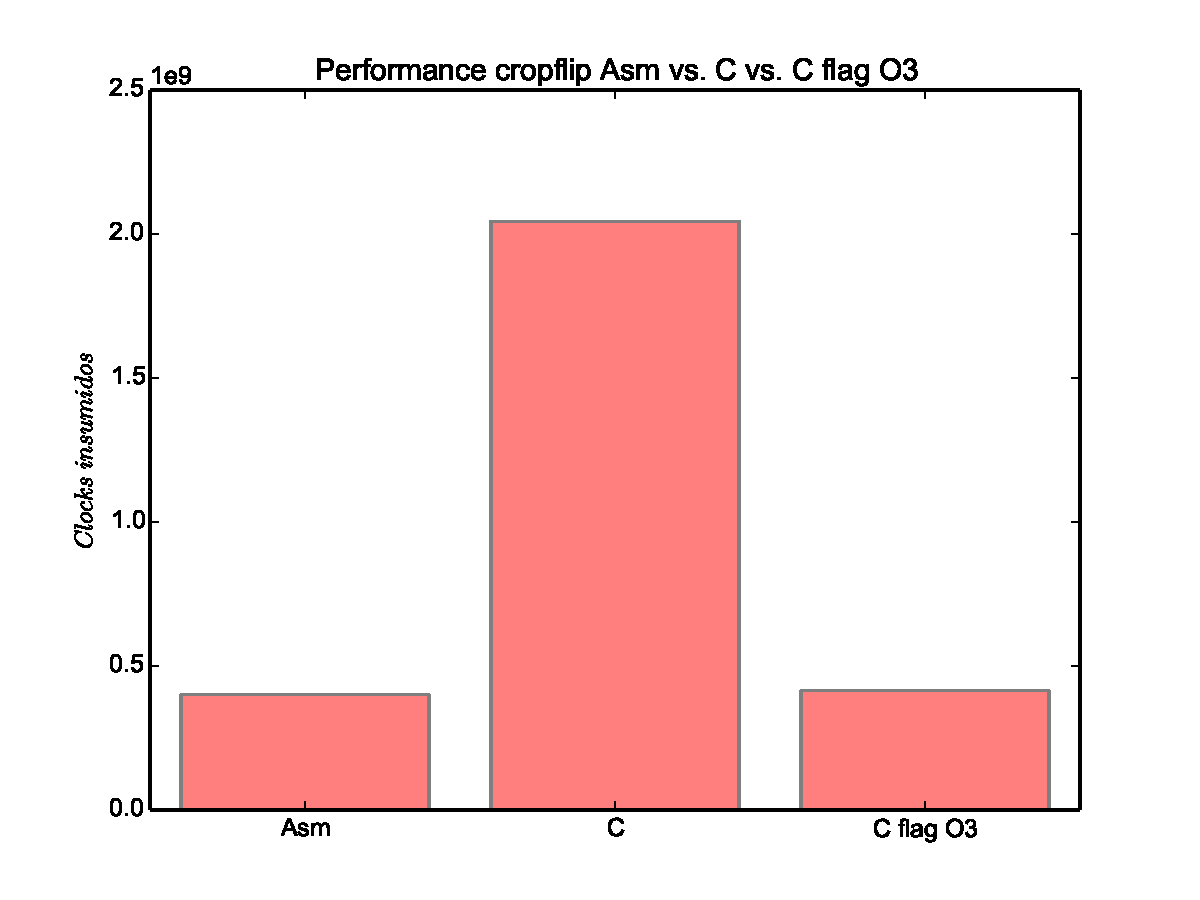
\includegraphics[scale=0.5]{cropflip.pdf}
	%\caption{La última de Star Wars}
  \end{center}
\end{figure}

Concluimos que los algoritmos escritos en $assembler$ son más rápidos quelos escritos en $C$. \\
Aunque podemos observar que en $C$ compilado con flag de optimizacion $O3$ llega a tener una performance muy similar.  \\

\newpage

\newpage

\subsection{Performance: cropflip vs. cache}
Para realizar el test, como se mencionó, se setea en el flag frio el valor uno para testear en frio y luego en cero para el test en calientes.
Se procesan 51 imágenes $lena32.bmp$ desde la resolución 424x424 con el id: 1 (539KB) aumentando de 16x16 hasta la resolución 1224x1224 con el id: 51 (4.5MB). Cada imágen se corre 100 veces y a cada muestra, que serán los tics de reloj totales para procesar la imágen, se la divide por el tamaño de la imágen, y se toma el promedio muestral intercuartil y el desvio estardar sobre la poda realizada.

\begin{figure}[h]
  \begin{center}
	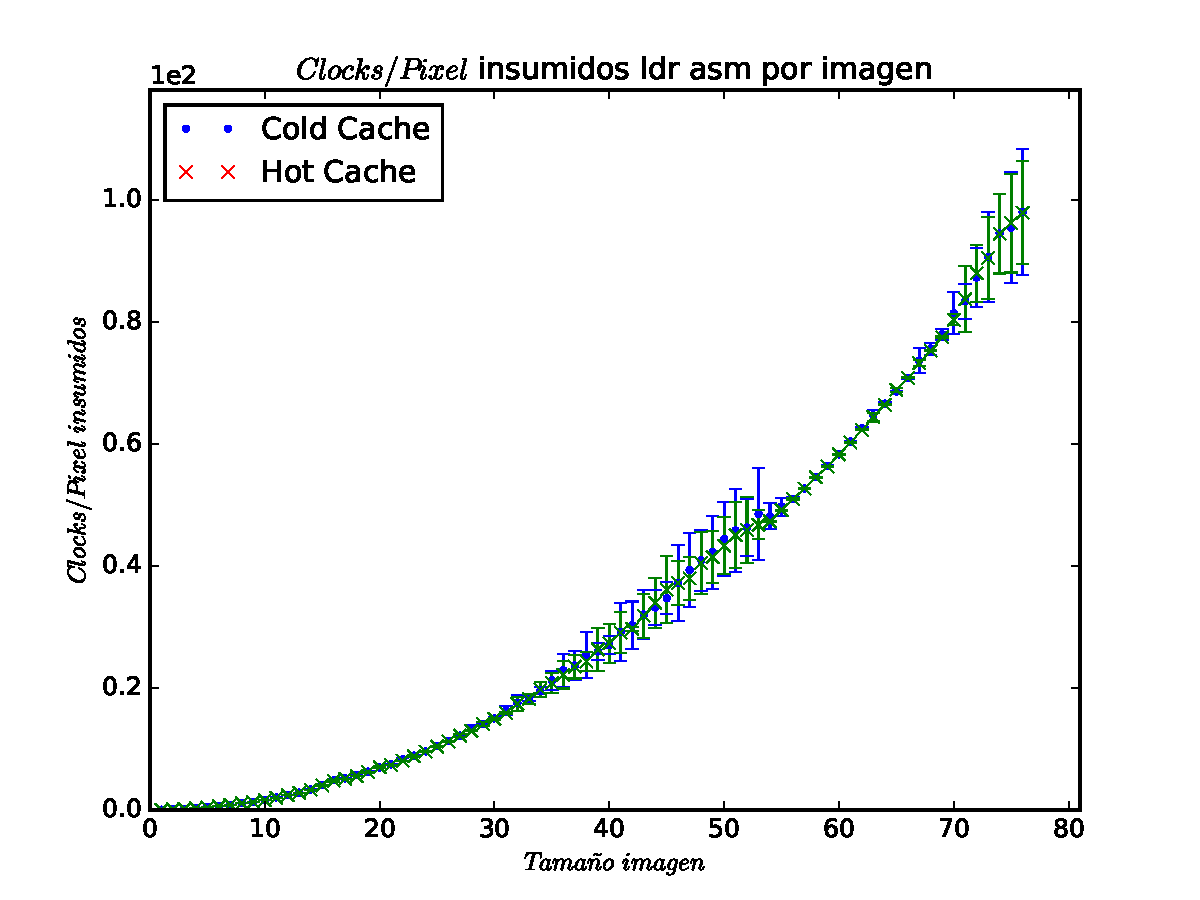
\includegraphics[scale=0.5]{ldrasmHotVsCold.pdf}
  \end{center}
\end{figure}

\begin{figure}[h]
  \begin{center}
	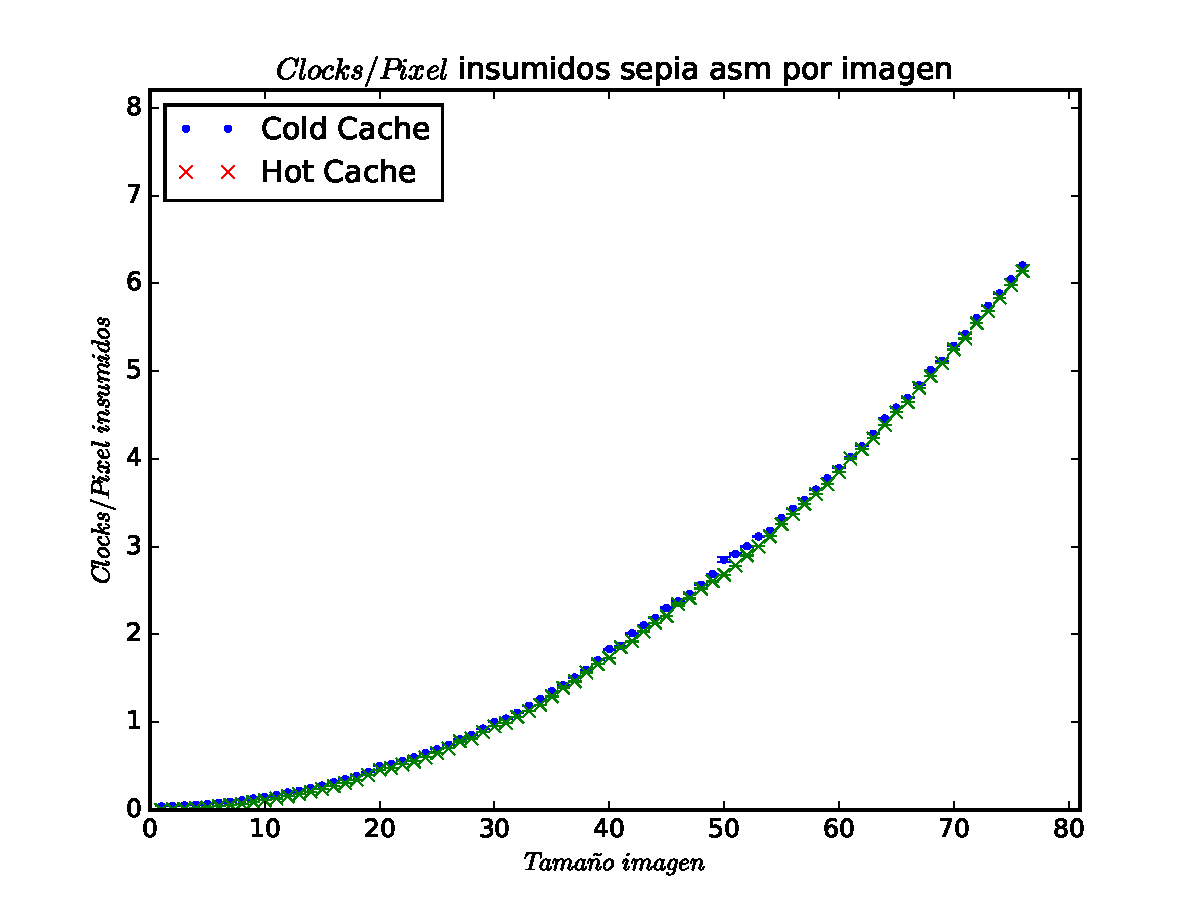
\includegraphics[scale=0.5]{sepiaasmHotVsCold.pdf}
  \end{center}
\end{figure}

\begin{figure}[h]
  \begin{center}
	\includegraphics[scale=0.5]{cropflipasmHotVsCold.pdf}
  \end{center}
\end{figure}

Podemos observar que salvo en $ldr$ todos los demás filtros mantienen el test de caché caliente por debajo del test en frio. Aunque por muy poca diferenca (menor al 0,2)
En principio esto es algo que tiene sentido. Una linea de caché tiene 64 bytes, por lo cual como ya hemos mencionado solo entrarn 16 pixeles en una linea. \\

Para el test en caliente las imágenes de menos de 3MB estarán completamente en memoria caché y tendremos 16/16 $hits$ = 100 $\%$ de $hits$ por linea. Es decir que nunca habrá necesidad de ir a buscar a memoria RAM pixeles de la imágen.\\ 
Para el test en frio lo que sucederá no es muy diferente. \\

Al no estar la imágen previamente en caché, el primer acceso será un $miss$ pero como el controlador caché utiliza el principio de localidad espacial traera a caché un bloque contiguo a una linea de la caché. Con lo cual los 15 accesos siguientes serán $hits$ por tendremos 15/16 $hits$ = 93,75 $\%$ de $hits$. 
Cuando la imágen supere el tamaño de la caché lo que puede estar sucediendo es que parte de la imágen esta en memoria caché, con lo cual se sigue obteniendo un rendimiento por debajo del test en frio.\\

El caso del filtro $ldr$ puede deberse a que las operaciones realizadas no dependen tanto de si la imágen está en caché o no. En particular, por como fué implementada la suma, el controlador caché podria estar desalojando y alojando lineas continuamente con lo cual no se beneficia tanto de las ventajas de esta memoria.


\newpage

\subsection{Performance: versiones de ldr}
\input{testSepia.tex}
\newpage

%\section{Conclusiones}
%Como pudimos comprobar, la importancia de SIMD para resolver este tipo de problematicas es muy significativa. 
Pudo observarse que los tiempos para un algoritmo en un lenguaje convencional como C son muy elevados llegando a requerir aproximadamente 4 veces mas de tiempo para realizar la misma tarea que en lenguaje assembler $($es decir que con assembler se obtiene una eficiencia del 400$ \% )$\\

Pudimos observar detalles particulares a cada implementacion. En especial, obtuvimos que para el filtro $ldr$ no era conveniente operar con enteros, pero esto parece estar mas asociado al tipo de implementacion y los cambios requeridos para lograr divisiones con enteros. Por ejemplo, si se hubiese realizado este mismo test sobre $sepia$ muy probablemente hubiese arrojado otros resultados debido a que operariamos con enteros sin perder paralelismo.\\

Otro resultado que pudimos observar tambien con el filtro $ldr$ es que los accesos a memoria no suponen un problema, dado que traer de a 4 o traer de a 1 es igual dado que la cache utiliza principio de vecinidad espacial y pedir 1 trae varios pixeles contiguos. La diferencia radica en poder realizar operaciones de forma paralela, siendo nuevamente este el punto fuerte de SIMD. \\




\end{document}

